\begin{figure}
	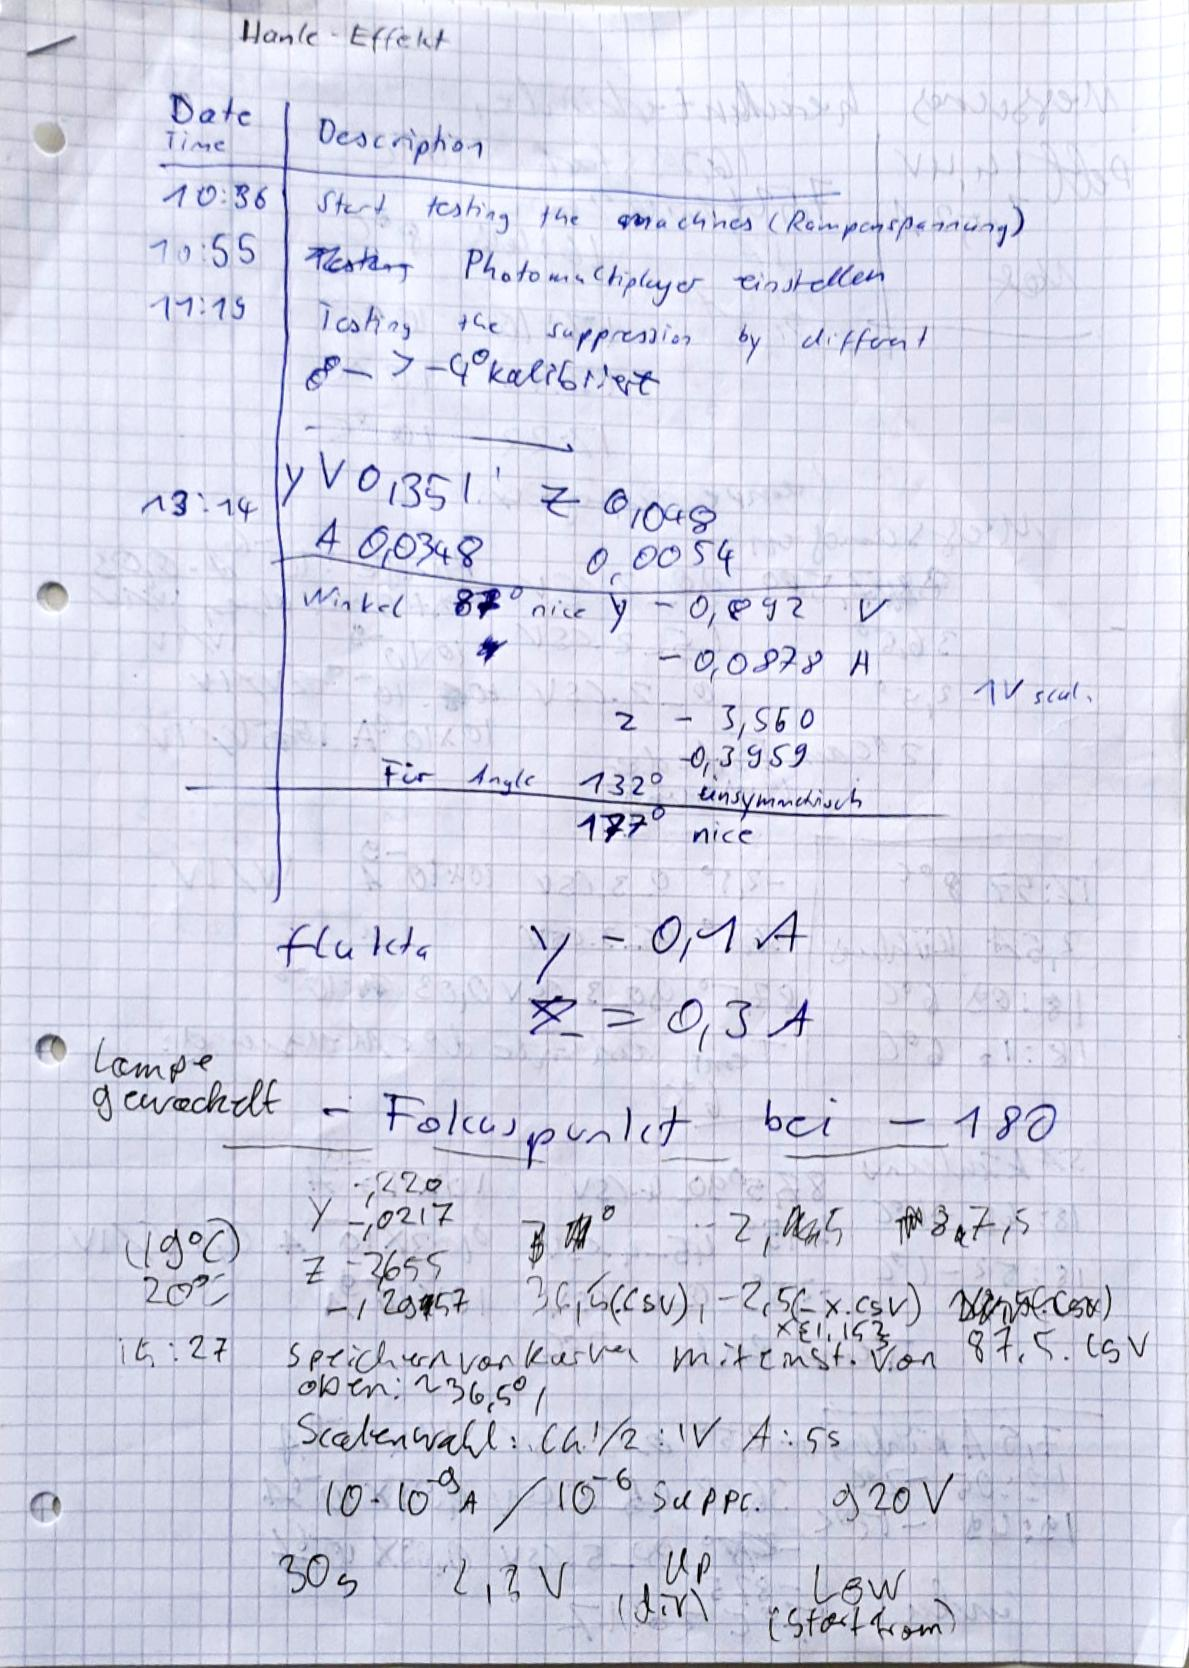
\includegraphics[scale=0.35]{Bild/Lab1}
	\centering
	\caption{Labor Aufschrieb}
\end{figure}
\begin{figure}
	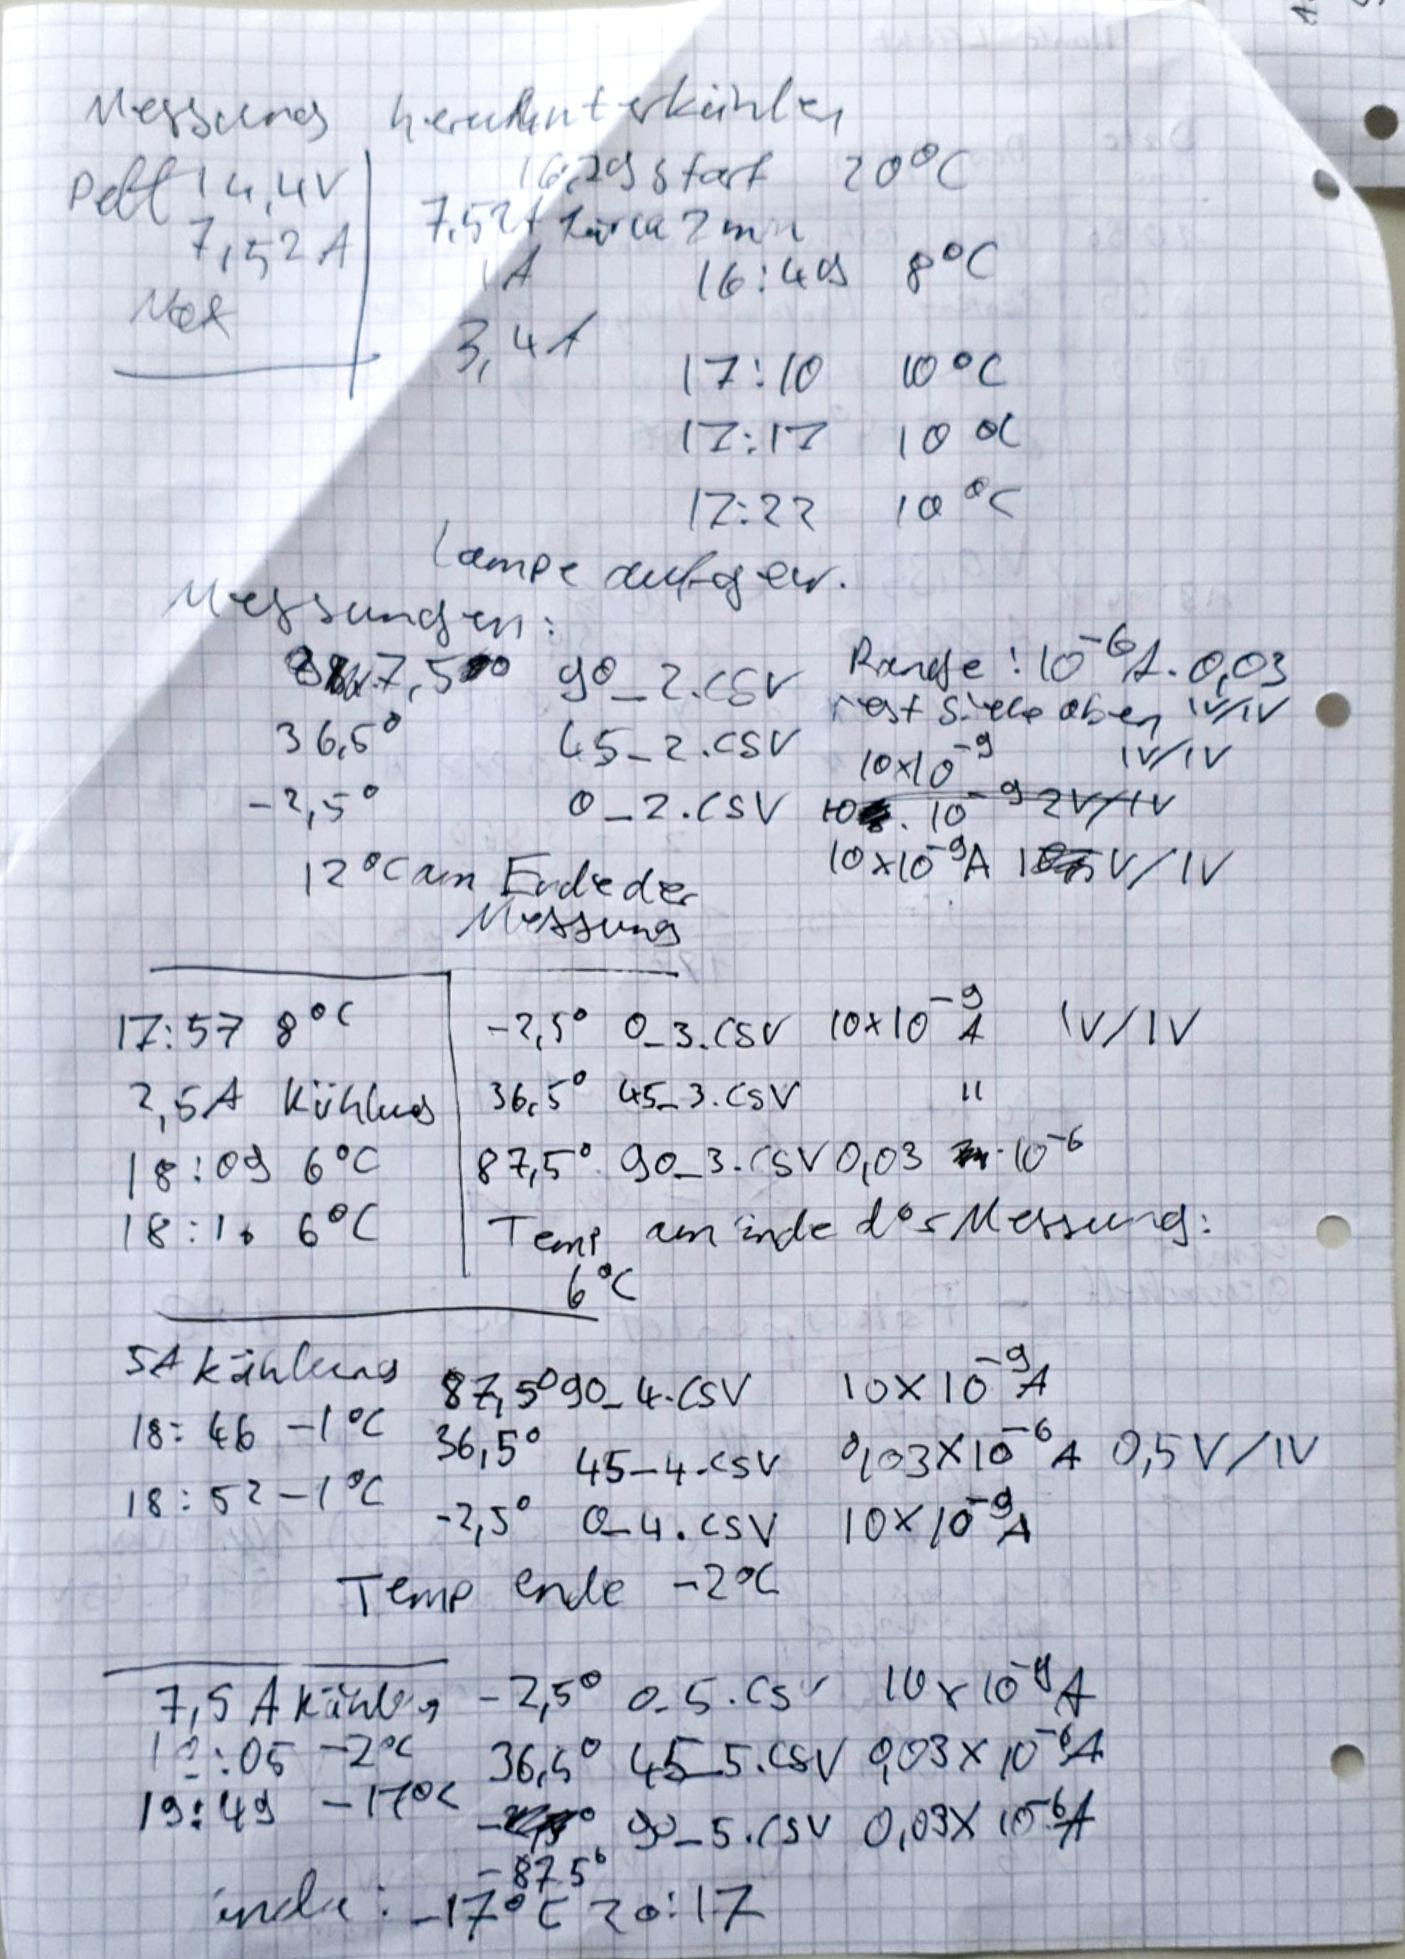
\includegraphics[scale=0.35]{Bild/Lab2}
	\centering
	\caption{Labor Aufschrieb}
\end{figure}
\begin{figure}
	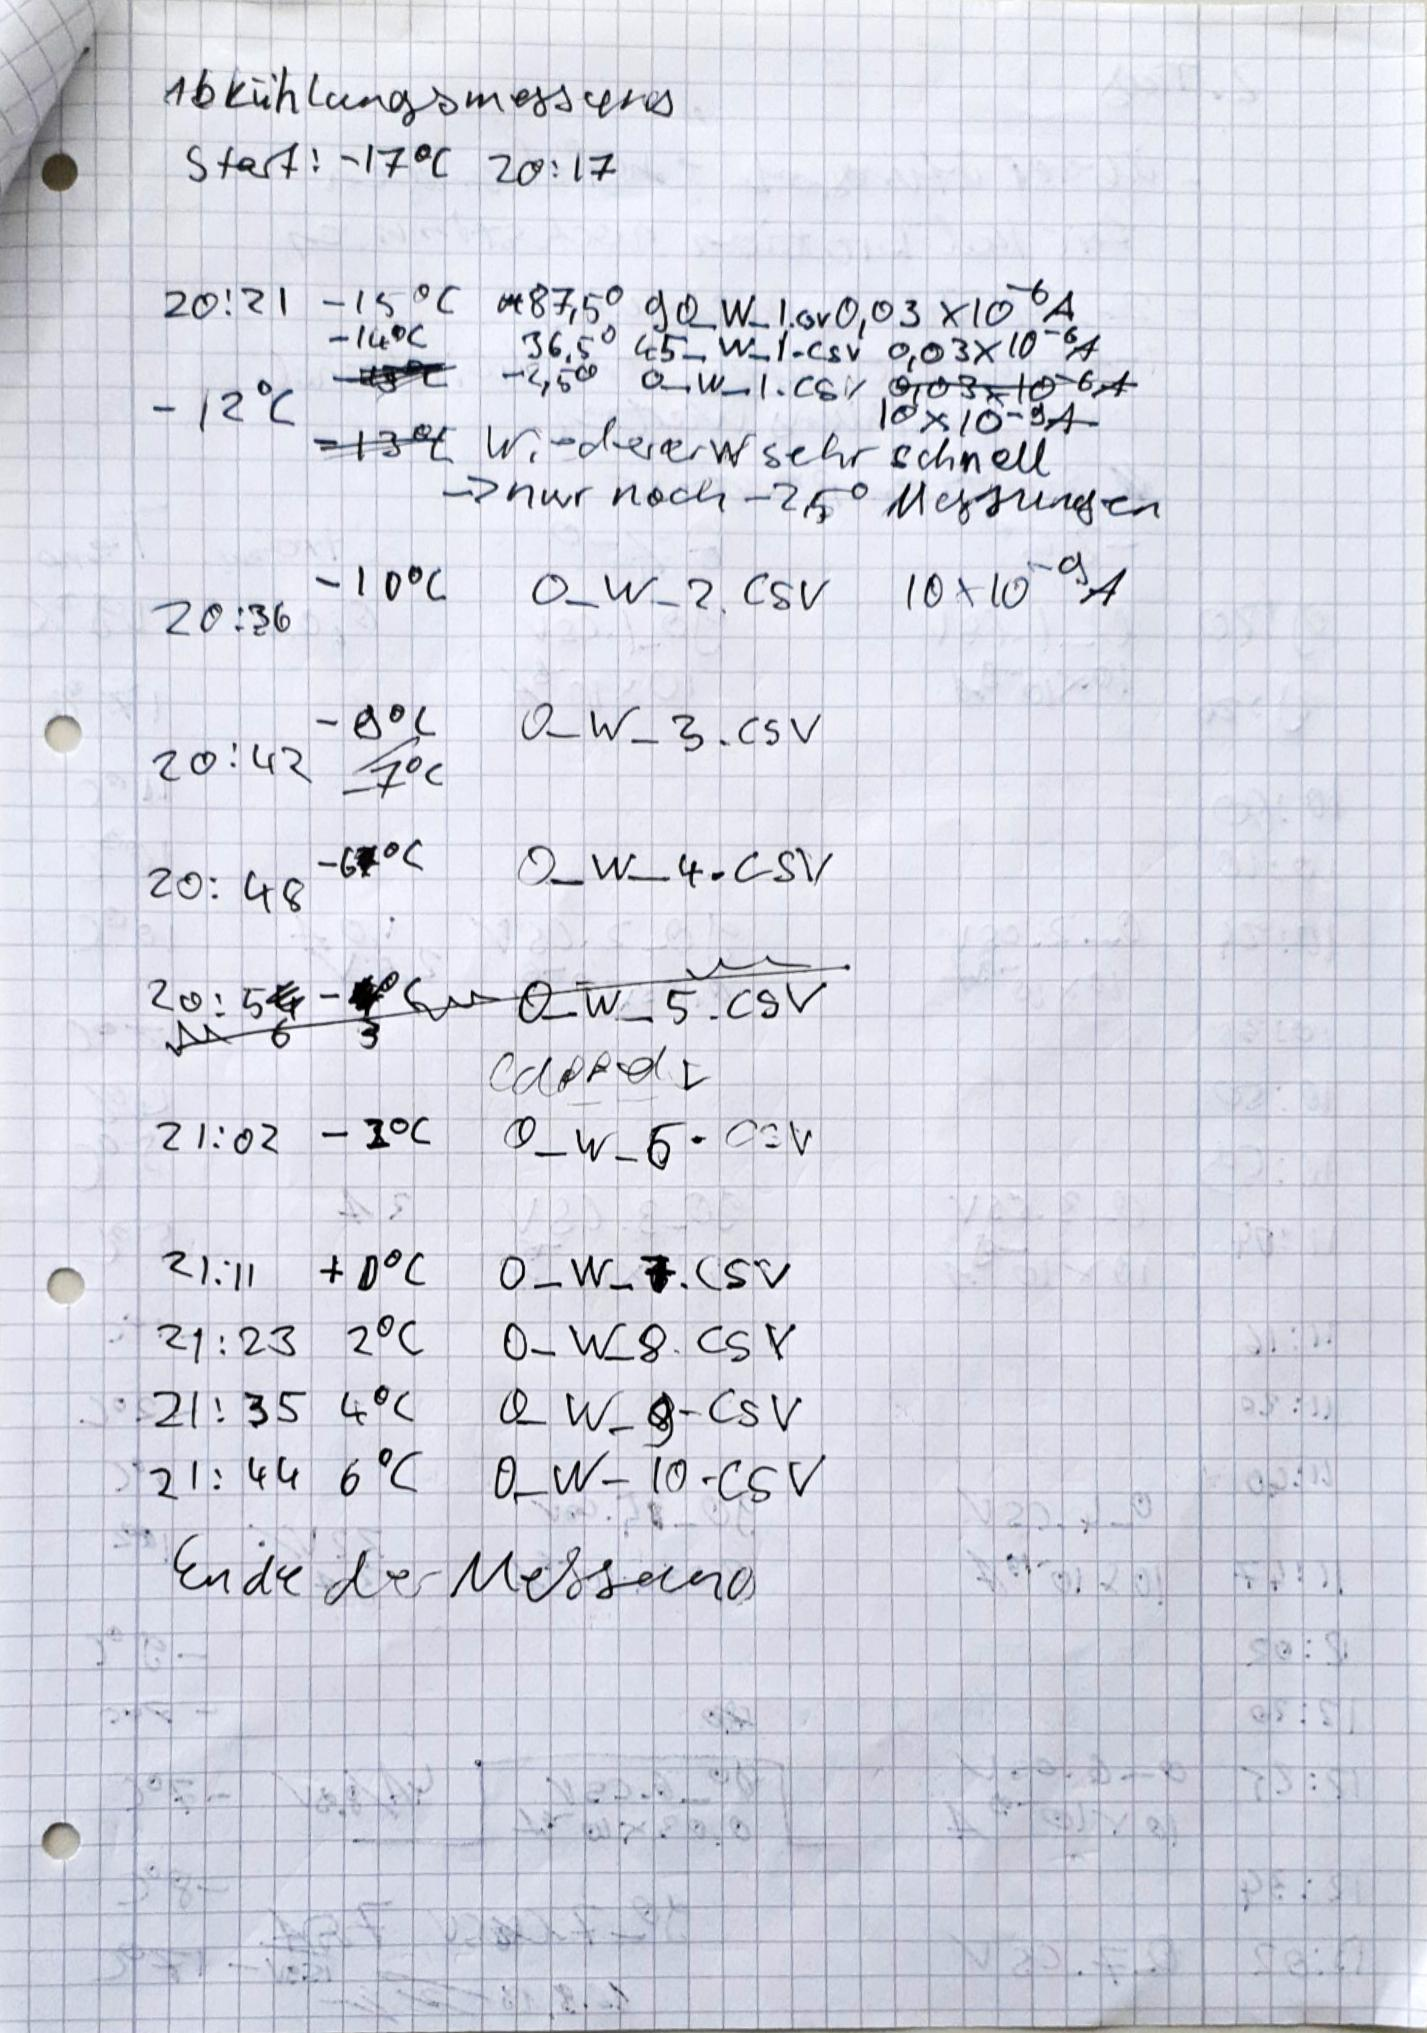
\includegraphics[scale=0.35]{Bild/Lab3}
	\centering
	\caption{Labor Aufschrieb}
\end{figure}
\begin{figure}
	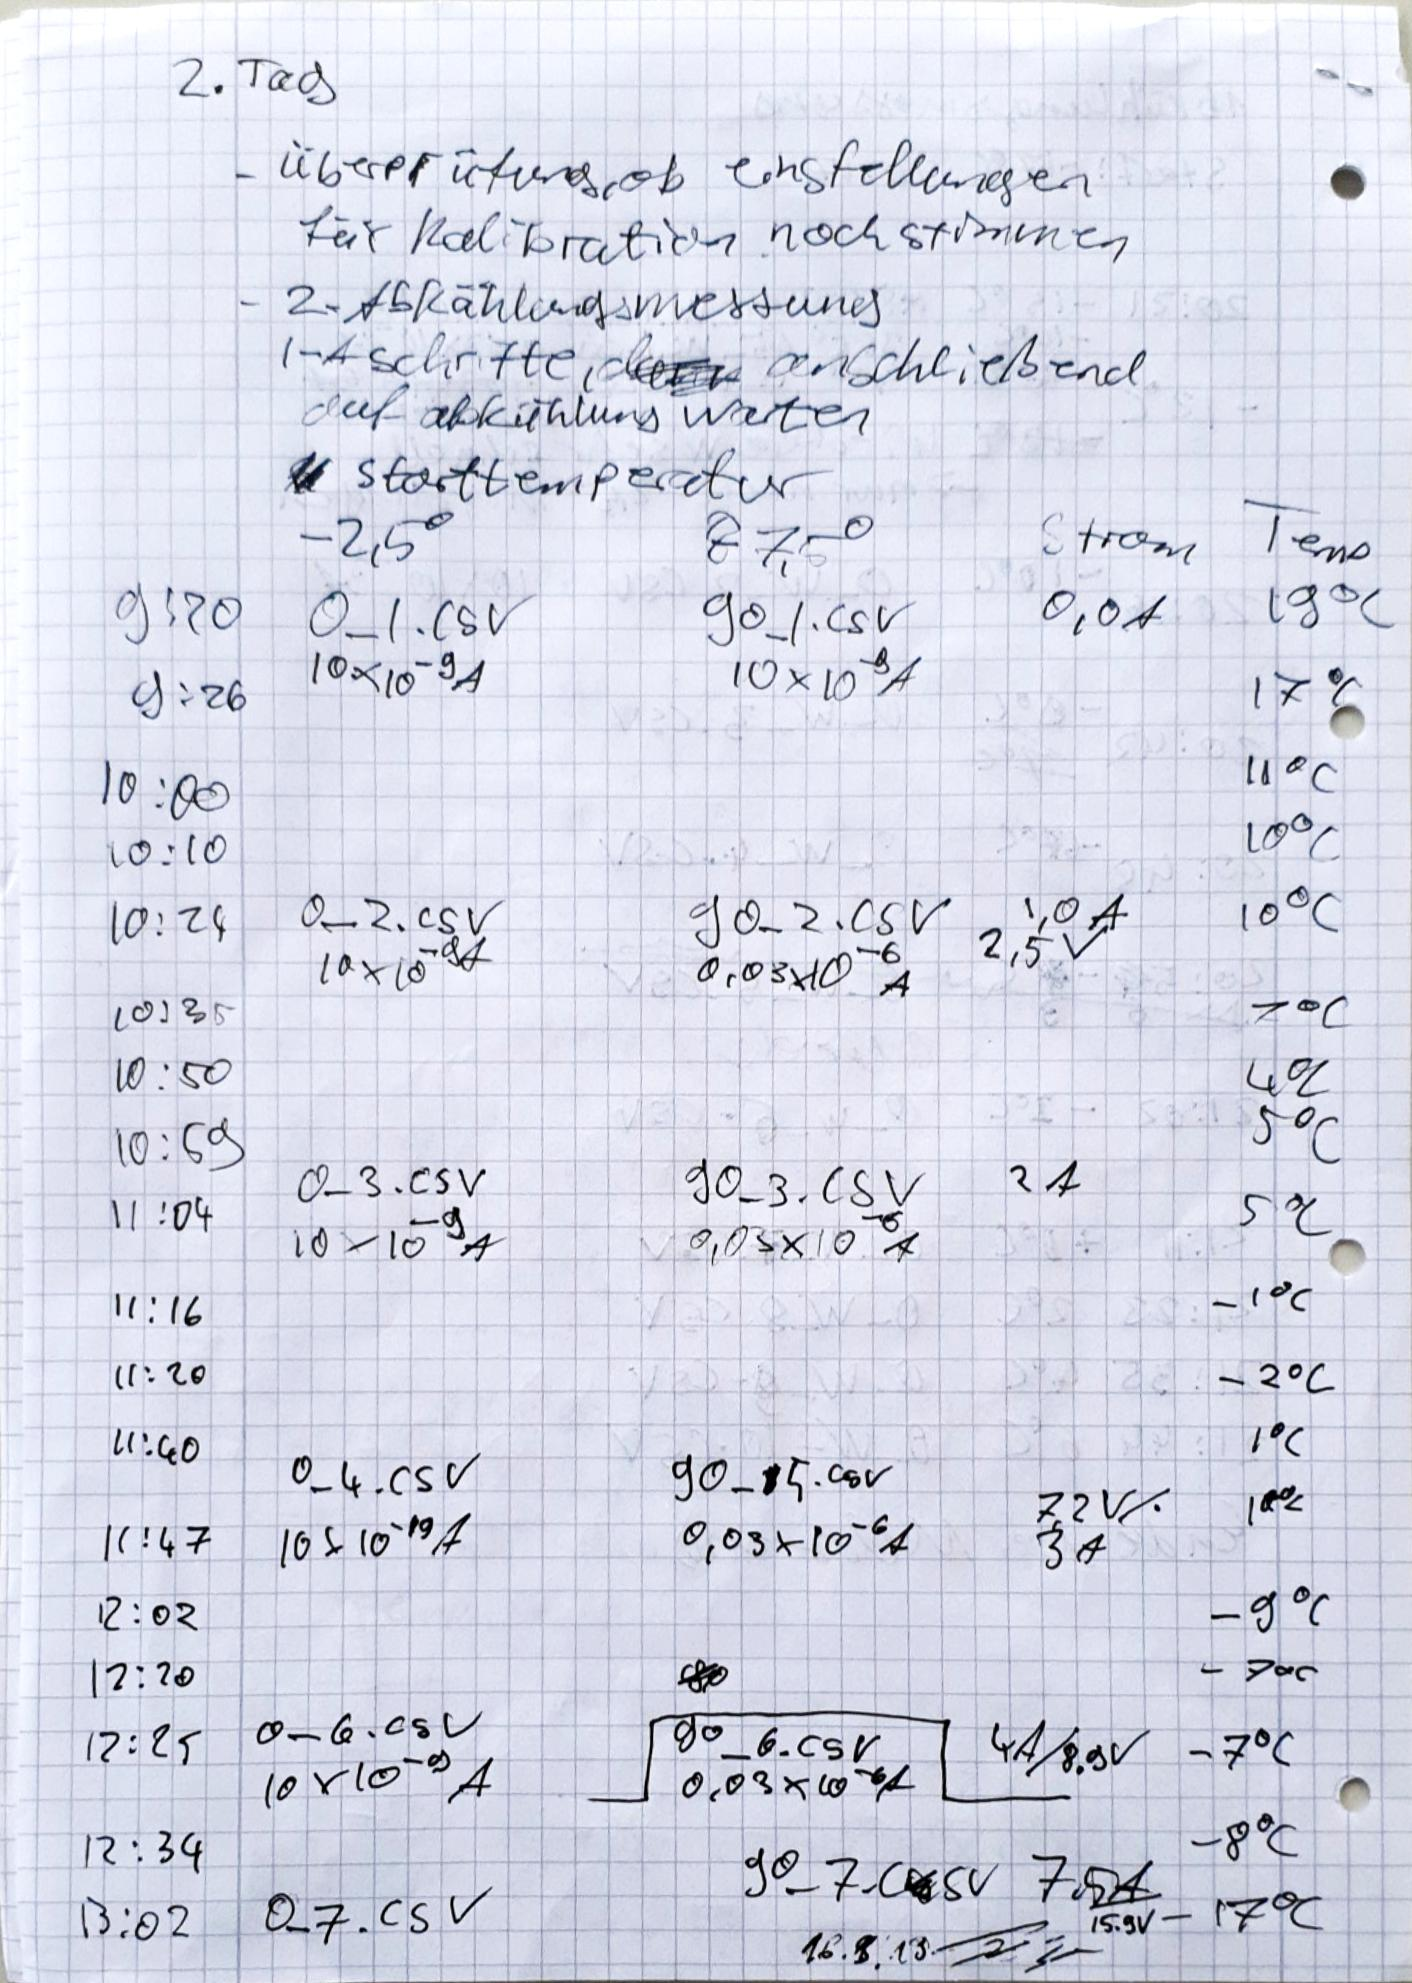
\includegraphics[scale=0.35]{Bild/Lab4}
	\centering
	\caption{Labor Aufschrieb}
\end{figure}




\begin{center}
	
		
		\begin{minipage}[t]{\textwidth}
			\begingroup
			\parfillskip=1pt
			% zwei weitere Minipages
			\begin{minipage}[t]{\textwidth}
				\includegraphics[scale=0.17]{Bild/Anhang/Statistik/stat(1)}
			\end{minipage}%
			\hfill
			\begin{minipage}[t]{\textwidth}
				\includegraphics[scale=0.17]{Bild/Anhang/Statistik/stat (2)}

			\end{minipage}%
			\par\endgroup
		\end{minipage}
	
\end{center}